\graphicspath{ {FutureWork/Images/} }


\chapter{Future Work}
\label{cha:futureWork}

\section{Introduction}
In this chapter we discuss some possible improvements or further research which are possible to add to the current approaches. \\
In section \ref{sec:generalization} we discuss a possible improvement on how we handled generalization of the medical data. In section \ref{sec:distributed}, we introduce a optimization which can be applied on our Word2Vec approaches by utilizing data distribution. In section \ref{sec:PatientClassification}, we explain a specific neural network which can use the found patterns by the Word2Vec approaches to predict or classify patients' disease trajectories.


\section{Generalization}
\label{sec:generalization}

In our Word2Vec approaches, we applied generalization on the medical states to reduce the amount of infrequent states. This was needed to retrieve more general n-grams. For this generalization, we divided some attributes into specific intervals. \\

Instead of dividing some attributes into specific intervals, we could apply normalization to it. Based on the distribution of the data, we can make more sensible intervals and assign them to the attributes.


\section{Distributed Word2Vec}
\label{sec:distributed}

Word2vec can be made distributed as the underlying idea is quite simplistic, it counts occurrences of n-grams. Counting occurrences based on labels, is a well known problem and is often solved by MapReduce algorithms \cite{mapreduce:article}. 


\section{Patient Classification}
\label{sec:PatientClassification}

As mentioned in section \ref{sec:word2vec}, a trained 2-layer neural network can be placed before another neural network and function as a lookup table. In this section, we discuss a possible neural network which allows us to further investigate the effectiveness of our Word2Vec approach to better classify patients. More concrete: we should check if a better accuracy is acquired with the lookup table in front of the neural network or without. 

\subsection{Problem Definition}
\label{sec:problem}

The medical history of a patient is seen as a time series with as datapoints EHRs. Based on the time series, we want to classify it into different disease trajectories. A patient who is classified into a specific disease trajectory, can be treated more specifically as we would have a better view what the next stages of the trajectory could be. \\

The medical data of multiple patients is a $3$ dimensional tensor, see figure \ref{fig:rnnData}. This data structure is the input structure for a neural network.

\begin{figure}[!htb]
	\centering
	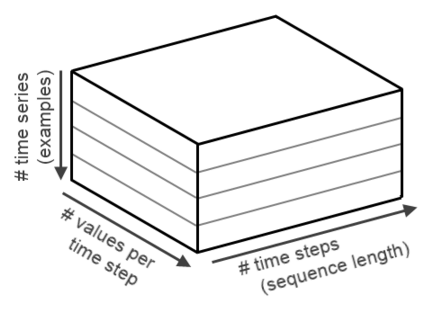
\includegraphics[width=0.8\textwidth]{rnnData.png}
	\caption{Overview of the data structure for medical data with a time aspect \cite{dl4jRnn:online}}
	\label{fig:rnnData}
\end{figure} 

Medical data has some problems which we will discuss.\\
It often consists of long time periods. This means there could be a long range of dependencies between events. In the context of training neural networks, this can cause a problem known as the vanishing gradient problem \cite{vanishingproblem:article}. \\
Patients do not have regular intervals in their medical data. The irregular intervals need to be transformed into regular intervals otherwise the time aspect will not be consistent throughout the data. \\
The standardization of the attributes needs to be taken into account. Preferably some sort of normalization should be applied as well. \\
Medical data has a high dimensionality. A lot of parameters need to be taken into account to retrieve accurate results. This causes a well known problem: Curse of Dimensionality \cite {curseofdim:book}. It causes the data to be sparse and have more infrequent cases. Therefore, more data is needed to cover all cases. Especially in medical data where outliers are important. 


\subsection{Approach}

Here we describe our approaches for the problems mentioned in the previous section. \\
We solve the vanishing gradient problem with a special form of recurrent neural network, see section \ref{sec:lstm}. \\
By applying our Word2Vec approach, the input is projected on another vector space using a lookup table. This vector space causes normalization. The standardization is also done in our Word2Vec approach. \\
As we mentioned, the Curse of Dimensionality causes the need for more data. The neural network in section \ref{sec:rnn} often handles high dimensional data \cite{nn1:article} \cite{nn2:article} \cite{nn3:article} \cite{nn4:article}. In a sense, because it keeps track of the time aspect of the data, it uses the data more thoroughly and thus handles the high dimensionality better. \\

A lot of these problems are covered in an extensive work of Graves et al \cite{gravesLstm:thesis} about using advanced neural networks to label sequences.

\subsubsection{Padding and Masking}
The transformation of irregular intervals into a regular ones, is done with padding and masking. \\

If we do not use any masking and padding, our data can only be of equal length sequences and at each time step a classification label. Our data on the other hand, consists of several different length sequences and only has one label for each sequence, namely the classification of the whole sequence. \\

The method of padding is simple. It adds empty events (ex. zeros) to the shorter sequences until all sequences are of equal length for both input and output. \\
Using padding, changes the data quite drastically and would cause problems during the training because of that. For this problem we use the method of masking. With masking, we have two additional arrays which contain the information about whether an input or output is padding or not. See figure \ref{fig:masking}, picture $2$ shows how the masking is done for a many to one case (which is the case that corresponds to labeling a complete sequence). 

\begin{figure}[!htb]
	\centering
	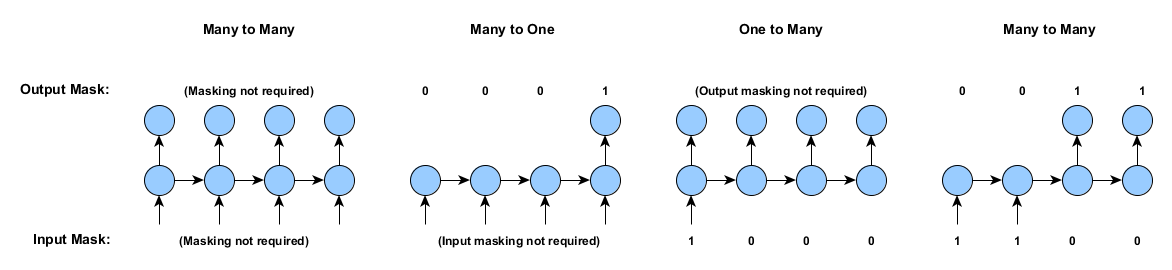
\includegraphics[width=\textwidth]{masking.png}
	\caption{Multiple masking methods \cite{dl4jRnn:online}}
	\label{fig:masking}
\end{figure} 


\subsection{Neural Network}
\label{sec:nn}

We still have to solve $2$ problems mentioned in section \ref{sec:problem}. \\
In this section we explain in more detail why Long-Short Term Memory (LSTM) \cite{lstmOrginin:article} networks handle the vanishing problem and long-term dependencies. \\

First we shortly repeat the structure of a neural network in figure \ref{fig:nnStructure}. We see the input $x$, different layers with their perceptrons, $\sigma$ as the activation function, and $y$ as output. 

\begin{figure}[!htb]
	\centering
	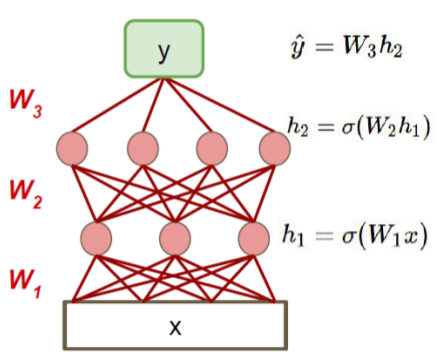
\includegraphics[width=0.7\textwidth]{nnStructure.png}
	\caption{General structure of a neural network \cite{IMECJaak}}
	\label{fig:nnStructure}
\end{figure} 

\subsubsection{Recurrent Neural Network}
\label{sec:rnn}

A standard neural network does not have any persistence. They will classify their input but when they get a stream of inputs (ex. speech), they will classify each word independently of each other and without any regards of the previous words. A recurrent neural network (RNN) addresses this problem by introducing networks with loops \cite{rnnOrigin:article}. This way, the output of a previous input has effect on the next input. In figure \ref{fig:rnnLoops}, we transform those loops into multiple copies of the same network which makes it easier to reason about. \\

\begin{figure}[!htb]
	\centering
	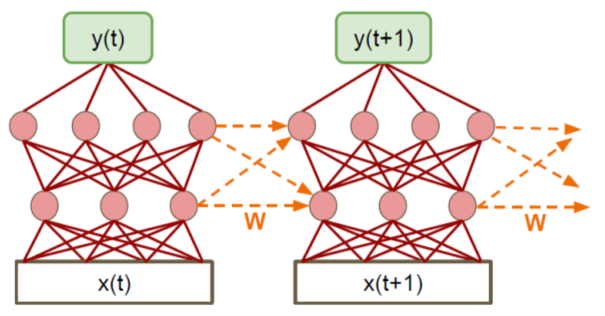
\includegraphics[width=0.7\textwidth]{rnnLoops.png}
	\caption{Unrolled recurrent neural network \cite{IMECJaak}}
	\label{fig:rnnLoops}
\end{figure} 

The problem with RNNs is mainly that they have trouble learning long-term dependencies which is often essential in time series \cite{longDepRNN:article}.


\subsubsection{Long Short Term Memory}
\label{sec:lstm}

A LSMT network is a specific RNN which is capable of learning long-term dependencies \cite{lstmDep:thesis}. We will explain the difference with a standard RNN and why a LSTM can learn these long-term dependencies. \\

A recurrent network is, as we said, a chain of connected neural networks. Those networks can have a simple structure like a single $tanh$ layer, see figure \ref{fig:rnnTanh}. \\

\begin{figure}[!htb]
	\centering
	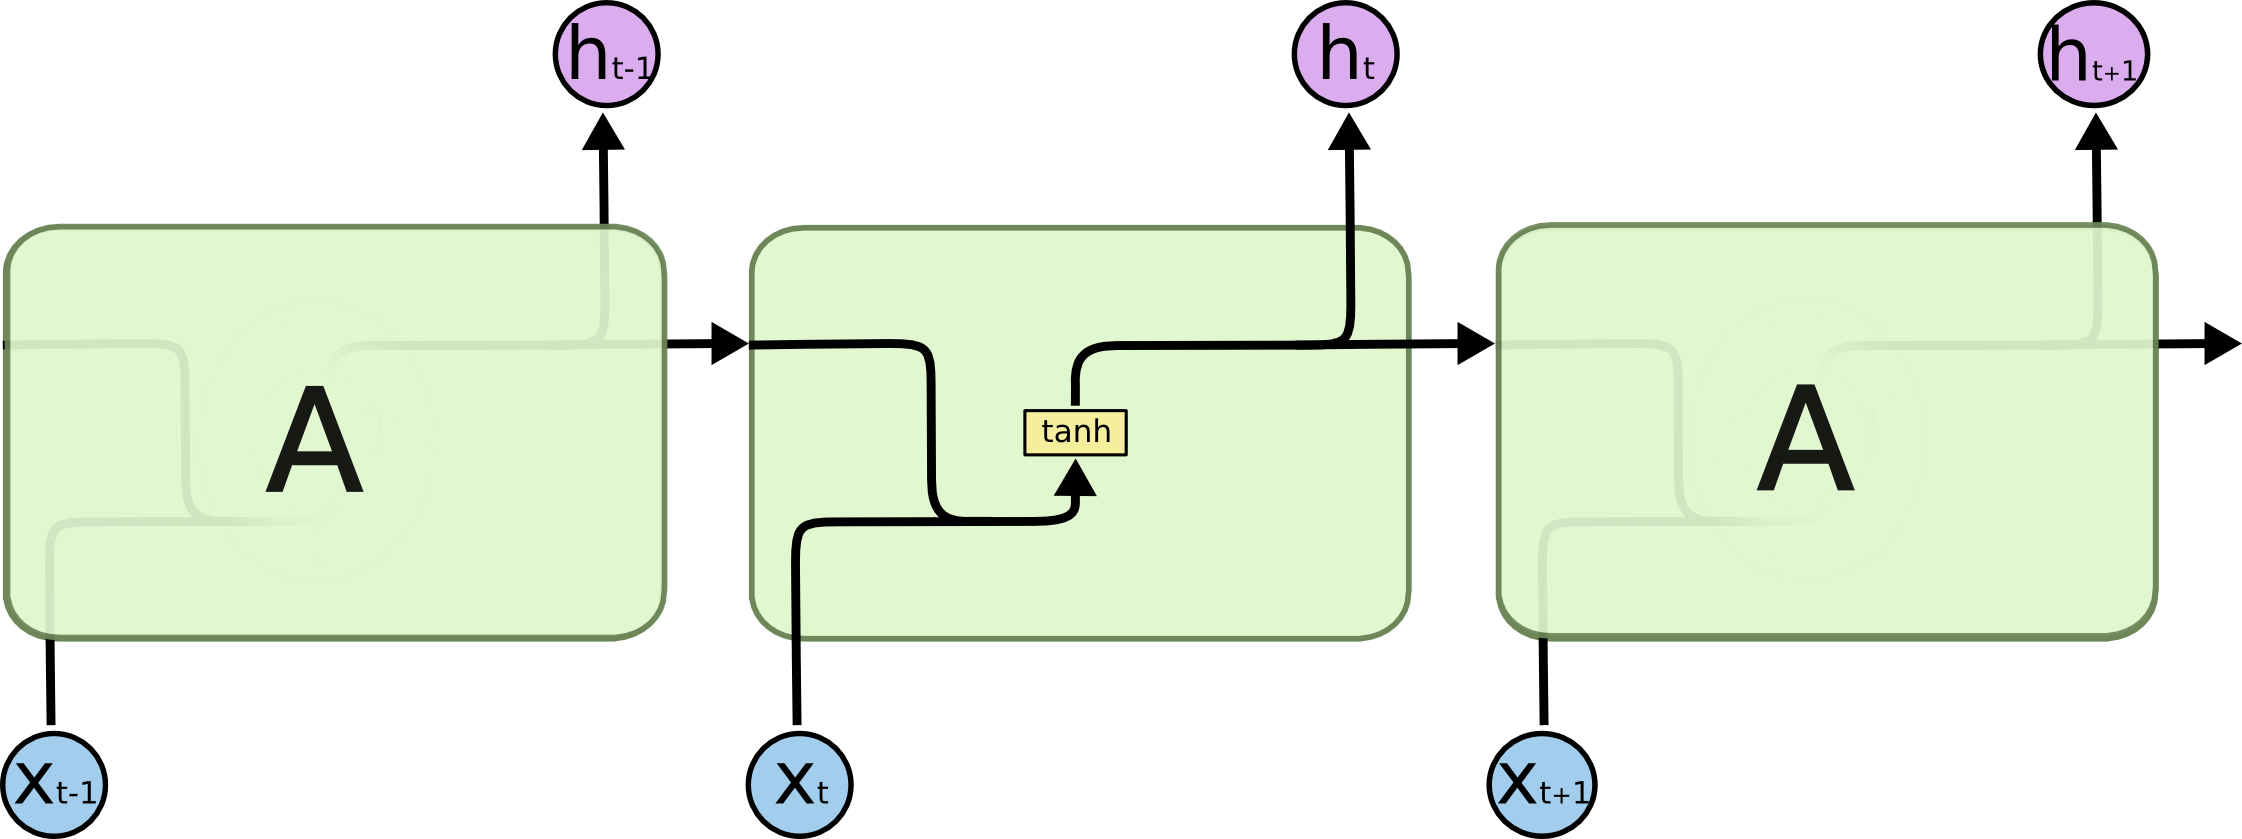
\includegraphics[width=0.7\textwidth]{rnnTanh.png}
	\caption{Unrolled recurrent neural network with a single tanh layer \cite{lstmGood:online}}
	\label{fig:rnnTanh}
\end{figure} 

It is important to see the difference with a LSTM. The repeating network does not have a single neural network layer, but has $4$ layers which each fulfills a specific goal, see figure \ref{fig:LSTMChain}.\\

\begin{figure}[!htb]
	\centering
	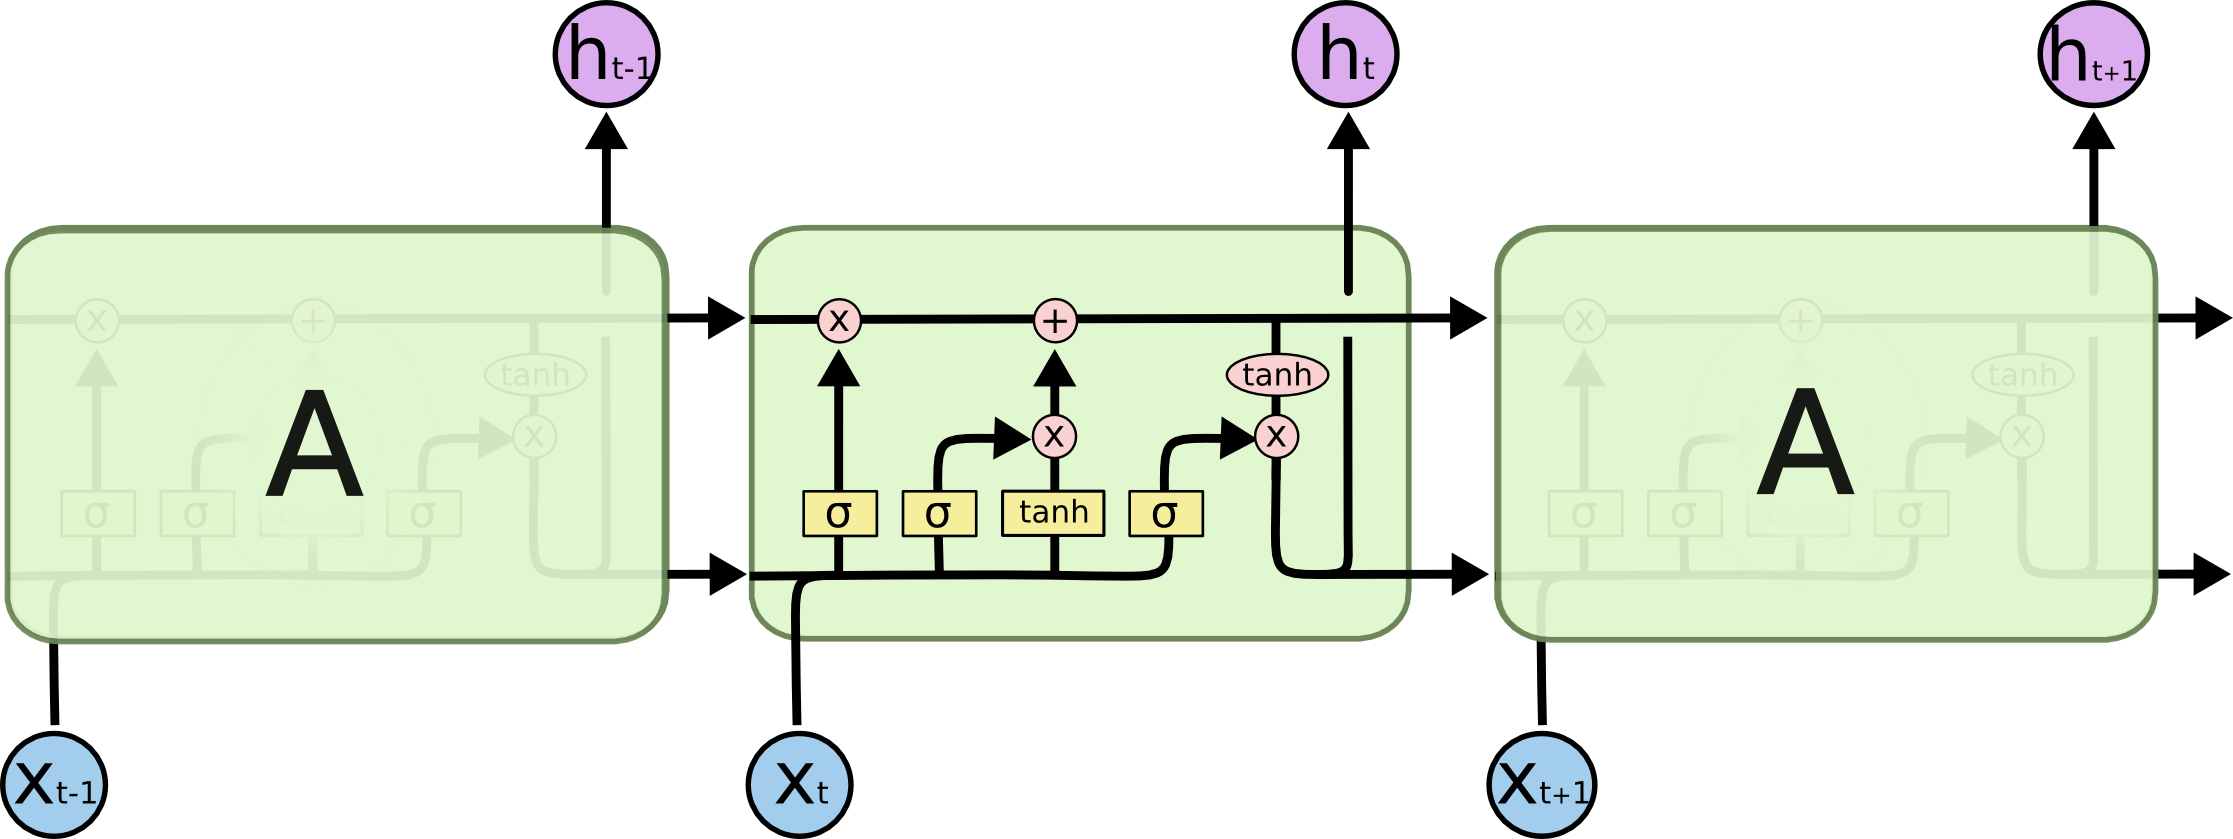
\includegraphics[width=0.7\textwidth]{LSTMChain.png}
	\caption{Unrolled LSTM network where each network has 4 layers \cite{lstmGood:online}}
	\label{fig:LSTMChain}
\end{figure} 

The main idea behind LSTM is that each repeated network has its own cell state. It functions as a  memory which can be updated with each new input. On figure \ref{fig:LSTMConveyor}, you can see the cell state $C$ through time. It can be compared with a conveyor belt which interacts with the input at certain gates. This way the state is updated throughout several inputs and this way a LSTM can keep track of long-term dependencies. \\

\begin{figure}[!htb]
	\centering
	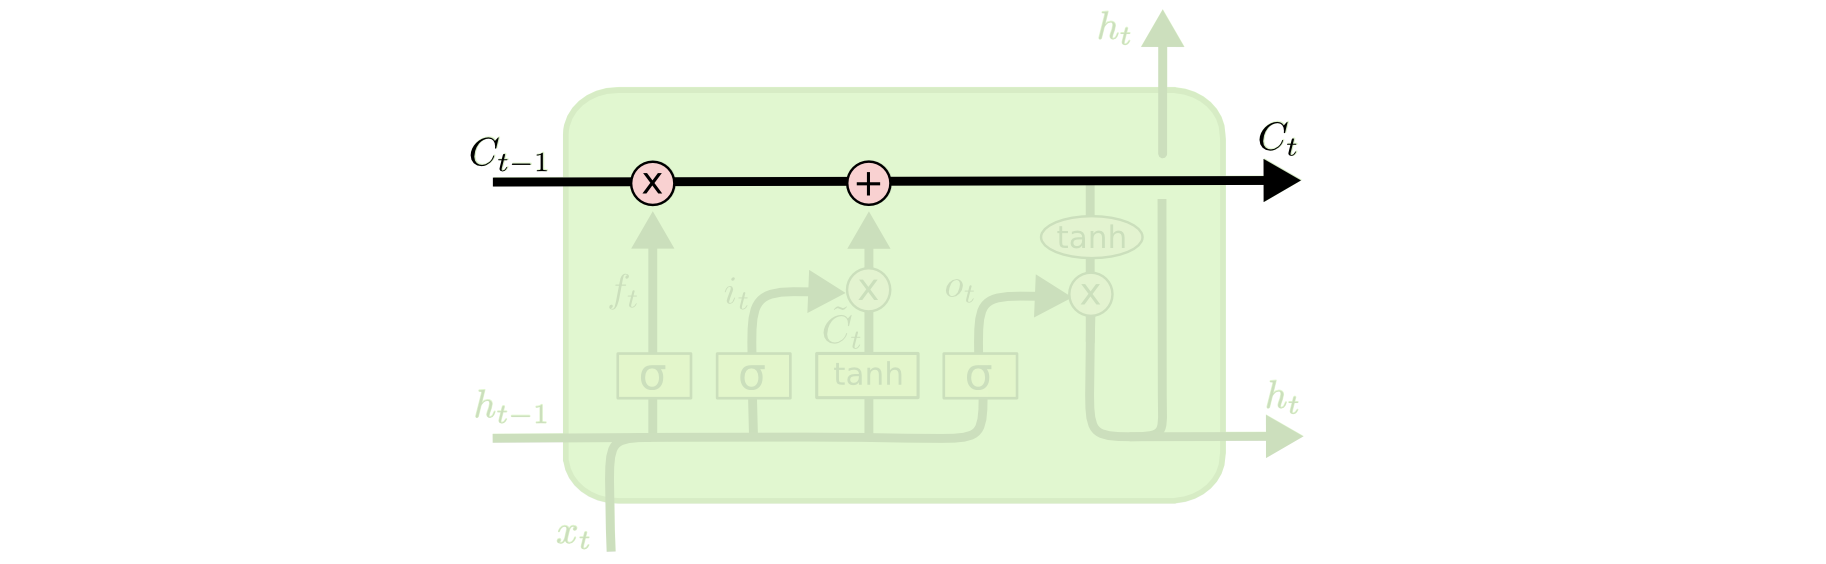
\includegraphics[width=0.7\textwidth]{LSTMConveyor.png}
	\caption{Representation of the cell state for a LSTM network \cite{lstmGood:online}}
	\label{fig:LSTMConveyor}
\end{figure} 

In the following figures, we show the different gates and their functions in changing the cell state depending on the input and the output of the previous network. Next to each figure, the formulas are shown on how the cell state is updated. There should be no surprises as they are not much different than the standard formulas of neural networks. \\

We start with the forget gate layer of a LSTM. Based on $x_t$ and $h_{t-1}$, it outputs a number between $0$ and $1$ for each number in the cell state $C_{t-1}$. This is shown in figure \ref{fig:LSTM1}. When the output is a $0$, the number in the cell state is completely erased. With the output $1$, the number does not change. \\

\begin{figure}[!htb]
	\centering
	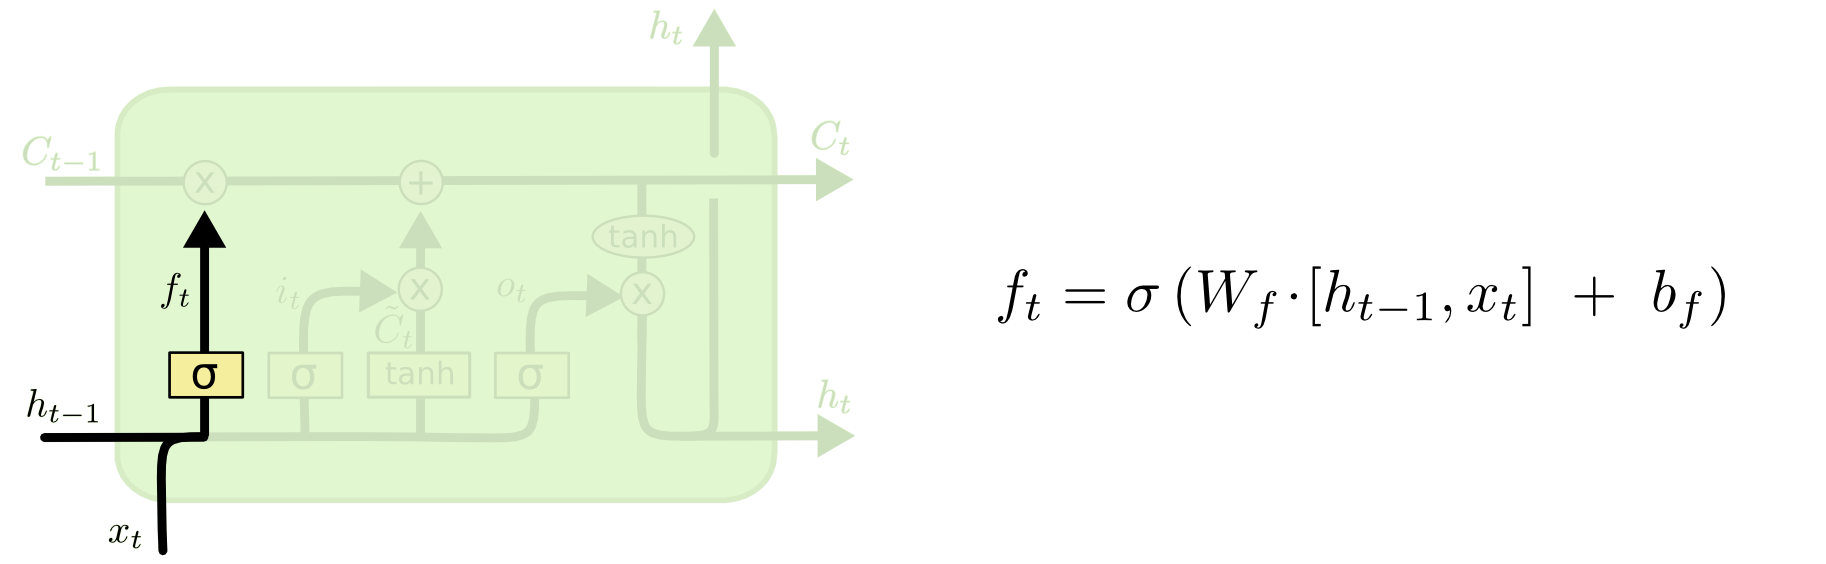
\includegraphics[width=0.7\textwidth]{LSTM1.png}
	\caption{Forget layer of a LSTM network \cite{lstmGood:online}}
	\label{fig:LSTM1}
\end{figure} 

Next we look to the input gate layer. This gate decides which values will be updated in the cell state and outputs those in $i_t$. It is then combined with the vector $\widetilde{C}_t$, which contains the new candidate values based on the input $x_t$ and $h_{t-1}$. This is shown in figure \ref{fig:LSTM2}. \\

\begin{figure}[!htb]
	\centering
	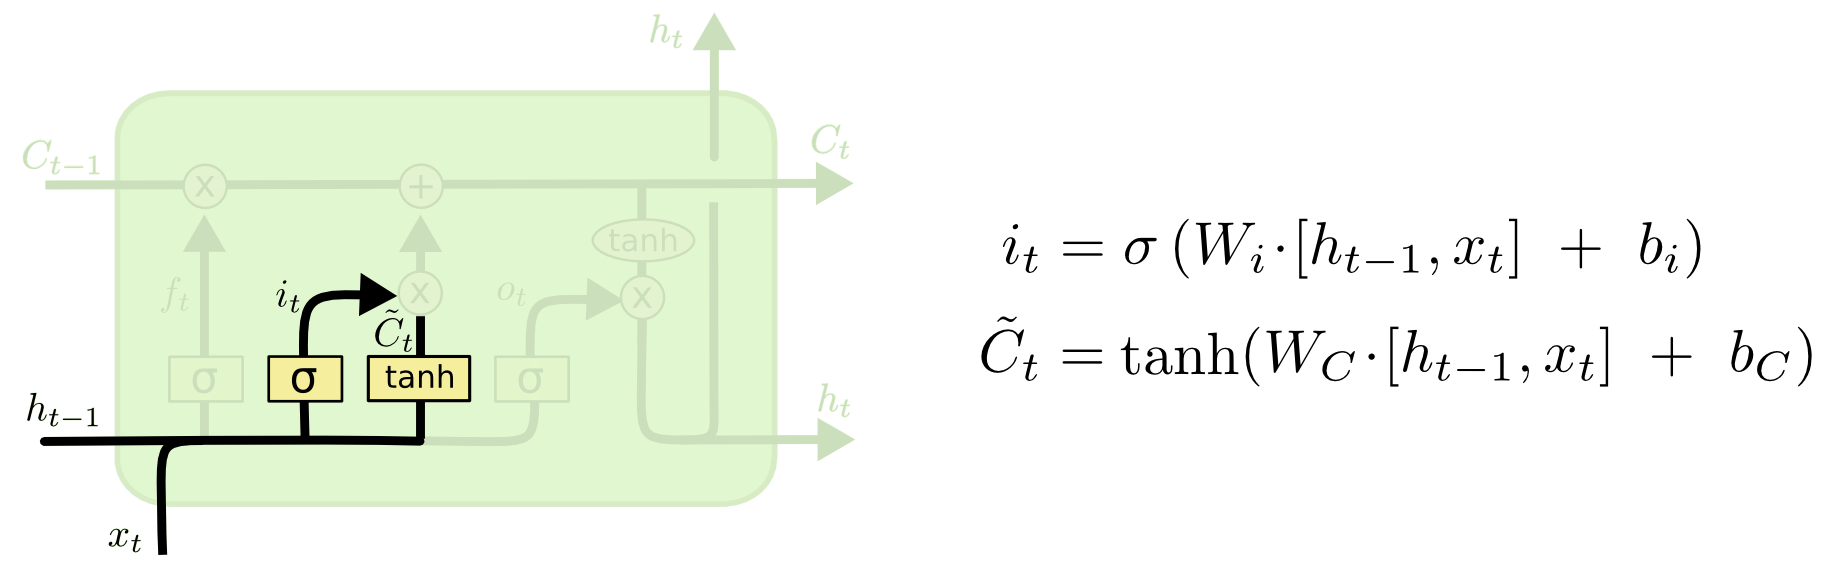
\includegraphics[width=0.7\textwidth]{LSTM2.png}
	\caption{Input layer of a LSTM network \cite{lstmGood:online}}
	\label{fig:LSTM2}
\end{figure} 

We can now combine the previous results and adjust the cell state. We multiply the old state with $f_t$ so we forget the needed elements. Then we add $i_t*\widetilde{C}_t$ which are the new candidate values multiplied by the amount on how much we want to update each state value. See figure \ref{fig:LSTM3}. \\

\begin{figure}[!htb]
	\centering
	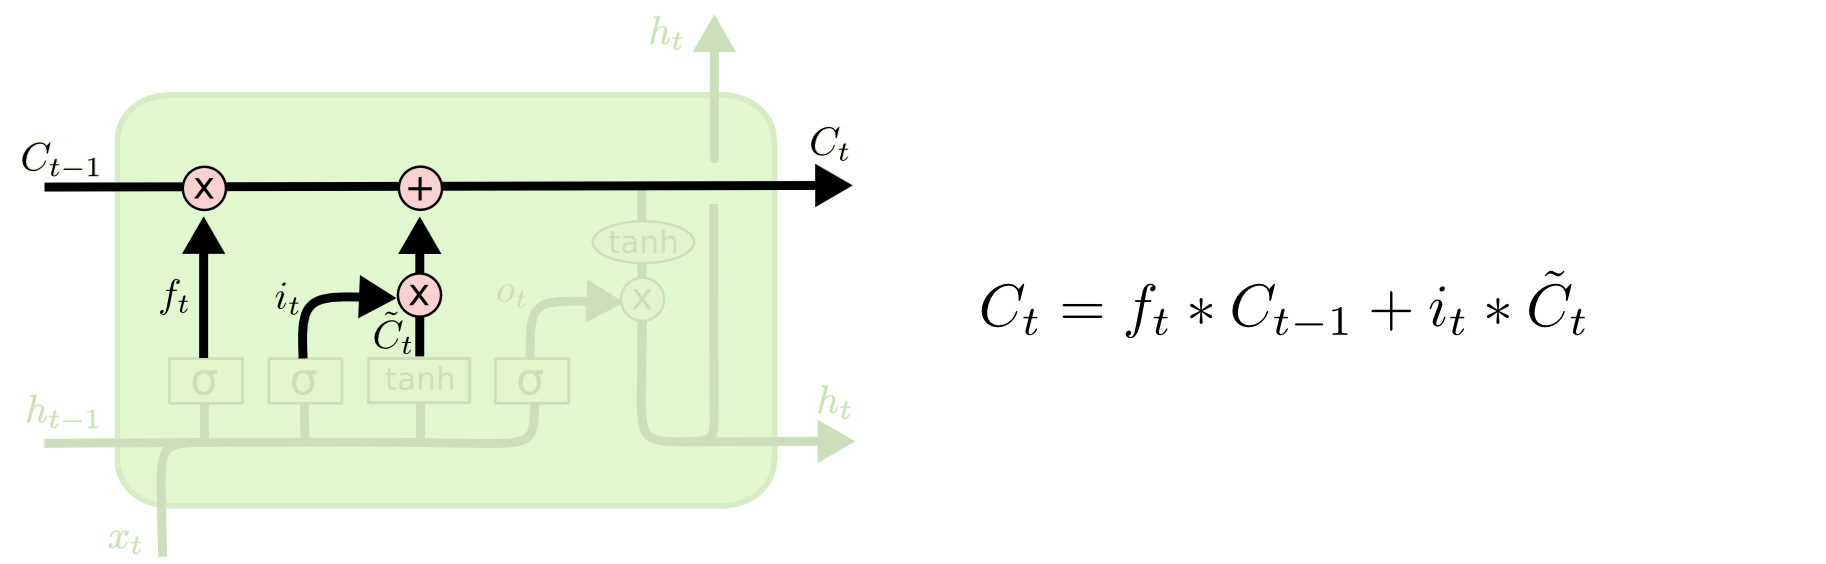
\includegraphics[width=0.7\textwidth]{LSTM3.png}
	\caption{Update process of the cell state of a LSTM network \cite{lstmGood:online}}
	\label{fig:LSTM3}
\end{figure} 

Finally, we need to output $h_t$ to the next network. This is based on the input and the cell state $C_t$. See figure \ref{fig:LSTM4}. \\

\begin{figure}[!htb]
	\centering
	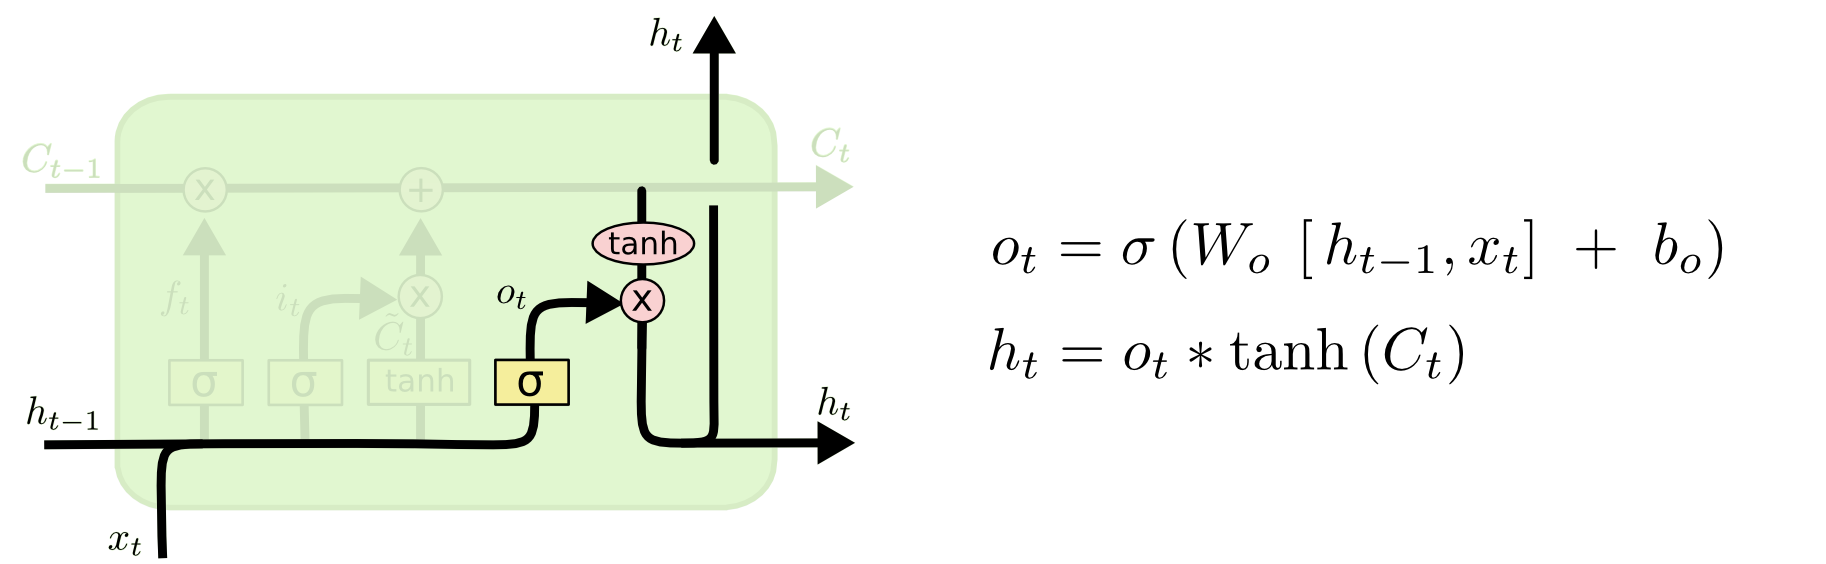
\includegraphics[width=0.7\textwidth]{LSTM4.png}
	\caption{Decide the output of a LSTM network \cite{lstmGood:online}}
	\label{fig:LSTM4}
\end{figure} 


\subsubsection{Variants Long Short Term Memory}

In "LSTM: A Search Space Odyssey" \cite{lstmSpace:article}, research is done between different variants of LSTM networks. It was concluded that the forget gate and the activation function are the most important. Other variants do not have a large influence and mainly add a lot of extra complexity.


\section{Conclusion}

Before this chapter, we already mentioned some possible roads to explore like a better disease code mapping strategy or extensive parameter tuning. \\

In this chapter we talked shortly about two possible improvements, a better generalization approach and a better use of data distribution to speed up to process. \\
We mainly focused on LSTM neural networks and explained why they should be suitable to predict or classify disease trajectories. They are able to handle the Curse of Dimensionality, long time dependencies, and take the time aspect of medical data into account. Our Word2Vec approaches can be used in combination with this kind of neural network. The prediction/classification accuracy of the LSMT neural network makes it possible to validate the working of our approaches by testing if the accuracy increases with the use of our Word2Vec approaches. \\


%%% Local Variables: 
%%% mode: latex
%%% TeX-master: "thesis"
%%% End: 
